\documentclass{standalone}
\usepackage[dvipsnames]{xcolor}
\usepackage{tikz}
\newcommand{\drawMineUnvisited}[1]{\draw [lightgray, fill=lightgray, fill opacity=0.5] #1 circle [radius=0.4]}
\newcommand{\drawMineFrontier}[1]{\draw [SkyBlue, fill=SkyBlue, fill opacity=0.5] #1 circle [radius=0.4]}
\newcommand{\drawMineVisited}[1]{\draw [orange, fill=orange, fill opacity=0.5] #1 circle [radius=0.4]}
\newcommand{\drawMineFound}[1]{\draw [green, fill=green, fill opacity=0.5] #1 circle [radius=0.4]}
\newcommand{\drawMineNotFound}[1]{\draw [black, fill=black, fill opacity=0.9] #1 circle [radius=0.4]}


\begin{document}
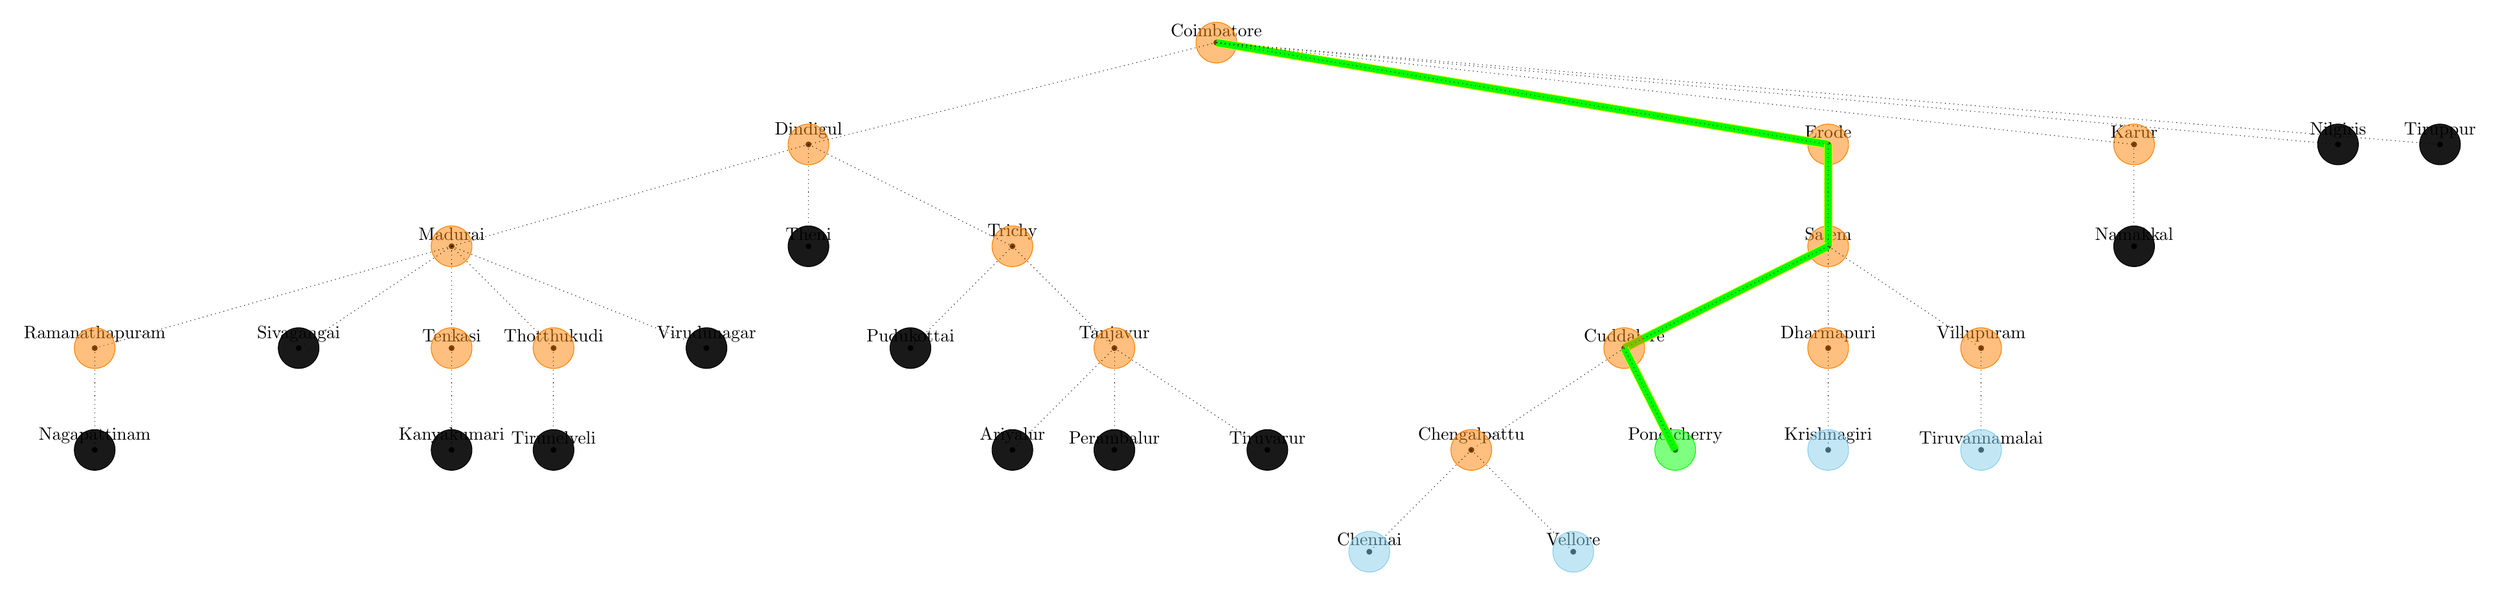
\begin{tikzpicture}
    \draw [black, fill=black ] (-18,0) circle [radius=0.05] node[above] {Coimbatore};
    \drawMineVisited{(-18,0)};

    %for coimbatore
    \draw [fill=black] (-26,-2) circle [radius=0.05] node[above] {Dindigul};
    \drawMineVisited{(-26,-2)};
    \draw [ dotted] (-18,0) -- (-26,-2);

    \draw [fill=black] (-6,-2) circle [radius=0.05] node[above] {Erode};
    \drawMineVisited{(-6,-2)};
    \draw [ dotted, preaction={%But before that
    draw,yellow,-,% Draw yellow without any arrow head
    double=green,
    double distance=10\pgflinewidth,
    }] (-18,0) -- (-6,-2);

    \draw [fill=black] (0,-2) circle [radius=0.05] node[above] {Karur};
	\drawMineVisited{(-0,-2)};
    \draw [ dotted] (-18,0) -- (-0,-2);

    \draw [fill=black] (4,-2) circle [radius=0.05] node[above] {Nilgiris};
	\drawMineNotFound{(4,-2)};
    \draw [ dotted] (-18,0) -- (4,-2);

    \draw [fill=black] (6,-2) circle [radius=0.05] node[above] {Tiruppur};
	\drawMineNotFound{(6,-2)};
    \draw [ dotted] (-18,0) -- (6,-2);

    %for dindigul
    % \draw [fill=black] (-25,-4) circle [radius=0.05] node[above] {Coimbatore};
    % \draw [fill=black] (-22,-4) circle [radius=0.05] node[above] {Karur};
    \draw [fill=black] (-33,-4) circle [radius=0.05] node[above] {Madurai};
	\drawMineVisited{(-33,-4)};
    \draw [ dotted] (-26,-2) -- (-33,-4);

    \draw [fill=black] (-26,-4) circle [radius=0.05] node[above] {Theni};
	\drawMineNotFound{(-26,-4)};
    \draw [ dotted] (-26,-2) -- (-26,-4);
    
    \draw [fill=black] (-22,-4) circle [radius=0.05] node[above] {Trichy};
	\drawMineVisited{(-22,-4)};
    \draw [ dotted] (-26,-2) -- (-22,-4);

    %for erode
    % \draw [fill=black] (-13,-4) circle [radius=0.05] node[above] {Coimbatore};
    \draw [fill=black] (-6,-4) circle [radius=0.05] node[above] {Salem};
	\drawMineVisited{(-6,-4)};
    \draw [ dotted, preaction={%But before that
    draw,yellow,-,% Draw yellow without any arrow head
    double=green,
    double distance=10\pgflinewidth,
    }] (-6,-2) -- (-6,-4);
    % \draw [fill=black] (-8,-4) circle [radius=0.05] node[above] {Tirrupur};

    %for karur
    % \draw [fill=black] (-4,-4) circle [radius=0.05] node[above] {Coimbatore};
    % \draw [fill=black] (-1,-4) circle [radius=0.05] node[above] {Dindigul};
    \draw [fill=black] (0,-4) circle [radius=0.05] node[above] {Namakkal};
    \draw [ dotted] (-0,-2) -- (-0,-4);
    \drawMineNotFound{(-0,-4)};
    % \draw [fill=black] (3,-4) circle [radius=0.05] node[above] {Trichy};

    %for niligirs
    % \draw [fill=black] (6,-4) circle [radius=0.05] node[above] {Coimbatore};

    %for Tiruppur
    % \draw [fill=black] (9,-4) circle [radius=0.05] node[above] {Coimbatore};
    % \draw [fill=black] (12,-4) circle [radius=0.05] node[above] {Erode};

    %for madurai
    \draw [fill=black] (-40,-6) circle [radius=0.05] node[above] {Ramanathapuram};
    \draw [ dotted] (-33,-4) -- (-40,-6);
    \drawMineVisited{(-40,-6)};

    \draw [fill=black] (-36,-6) circle [radius=0.05] node[above] {Sivagangai};
    \draw [ dotted] (-33,-4) -- (-36,-6);
    \drawMineNotFound{(-36,-6)};

    \draw [fill=black] (-33,-6) circle [radius=0.05] node[above] {Tenkasi};
    \draw [ dotted] (-33,-4) -- (-33,-6);
    \drawMineVisited{(-33,-6)};

    \draw [fill=black] (-31,-6) circle [radius=0.05] node[above] {Thotthukudi};
    \draw [ dotted] (-33,-4) -- (-31,-6);
    \drawMineVisited{(-31,-6)};

    \draw [fill=black] (-28,-6) circle [radius=0.05] node[above] {Virudunagar};
    \draw [ dotted] (-33,-4) -- (-28,-6);
    \drawMineNotFound{(-28,-6)};
    %for Theni

    %for Trichy
    \draw [fill=black] (-24,-6) circle [radius=0.05] node[above] {Pudukottai};
    \draw [ dotted] (-22,-4) -- (-24,-6);
    \drawMineNotFound{(-24,-6)};

    \draw [fill=black] (-20,-6) circle [radius=0.05] node[above] {Tanjavur};
    \draw [ dotted] (-22,-4) -- (-20,-6);
    \drawMineVisited{(-20,-6)};

    %for Salem
    \draw [fill=black] (-10,-6) circle [radius=0.05] node[above] {Cuddalore};
    \draw [ dotted, preaction={%But before that
    draw,yellow,-,% Draw yellow without any arrow head
    double=green,
    double distance=10\pgflinewidth,
    }] (-6,-4) -- (-10,-6);
    \drawMineVisited{(-10,-6)};

    \draw [fill=black] (-6,-6) circle [radius=0.05] node[above] {Dharmapuri};
    \draw [ dotted] (-6,-4) -- (-6,-6);
    \drawMineVisited{(-6,-6)};

    \draw [fill=black] (-3,-6) circle [radius=0.05] node[above] {Villupuram};
    \draw [ dotted] (-6,-4) -- (-3,-6);
    \drawMineVisited{(-3,-6)};

    %for Namakkal

    %for Ramanathapuram
    \draw [fill=black] (-40,-8) circle [radius=0.05] node[above] {Nagapattinam};
    \draw [ dotted] (-40,-6) -- (-40,-8);
    \drawMineNotFound{(-40,-8)};
    %for  Sivagangai

    %for Tenkasi
    \draw [fill=black] (-33,-8) circle [radius=0.05] node[above] {Kanyakumari};
    \draw [ dotted] (-33,-6) -- (-33,-8);
    \drawMineNotFound{(-33,-8)};

    %for Thoothukudi
    \draw [fill=black] (-31,-8) circle [radius=0.05] node[above] {Tirunelveli};
    \draw [ dotted] (-31,-6) -- (-31,-8);
    \drawMineNotFound{(-31,-8)};

    %for Virudunagar

    %for Pudukottai

    %for Tanjavur
    \draw [fill=black] (-22,-8) circle [radius=0.05] node[above] {Ariyalur};
    \draw [ dotted] (-20,-6) -- (-22,-8);
    \drawMineNotFound{(-22,-8)};

    \draw [fill=black] (-20,-8) circle [radius=0.05] node[above] {Perambalur};
    \draw [ dotted] (-20,-6) -- (-20,-8);
    \drawMineNotFound{(-20,-8)};

    \draw [fill=black] (-17,-8) circle [radius=0.05] node[above] {Tiruvarur};
    \draw [ dotted] (-20,-6) -- (-17,-8);
    \drawMineNotFound{(-17,-8)};

    %for Cuddalore
    \draw [fill=black] (-13,-8) circle [radius=0.05] node[above] {Chengalpattu};
    \draw [ dotted] (-10,-6) -- (-13,-8);
    \drawMineVisited{(-13,-8)};

    \draw [fill=black] (-9,-8) circle [radius=0.05] node[above] {Pondicherry};
    \draw [ dotted, preaction={%But before that
    draw,yellow,-,% Draw yellow without any arrow head
    double=green,
    double distance=10\pgflinewidth,
    }] (-10,-6) -- (-9,-8);
    \drawMineFound{(-9,-8)};

    %for Dharmapuri
    \draw [fill=black] (-6,-8) circle [radius=0.05] node[above] {Krishnagiri};
    \draw [ dotted] (-6,-6) -- (-6,-8);
    \drawMineFrontier{(-6,-8)};
    %for Villupuram
    \draw [fill=black] (-3,-8) circle [radius=0.05] node[above] {Tiruvannamalai};
    \draw [ dotted] (-3,-6) -- (-3,-8);
    \drawMineFrontier{(-3,-8)};
    %for Chengalpattur
    \draw [fill=black] (-15,-10) circle [radius=0.05] node[above] {Chennai};
    \draw [ dotted] (-13,-8) -- (-15,-10);
    \drawMineFrontier{(-15,-10)};
    \draw [fill=black] (-11,-10) circle [radius=0.05] node[above] {Vellore};
    \draw [ dotted] (-13,-8) -- (-11,-10);
    \drawMineFrontier{(-11,-10)};

\end{tikzpicture}
\end{document}


